%==============================================================================
% 9 RESULTS IV: CLOSED-LOOP PLAUSIBILITY
% Plano: a estrategia real jogando contra o gemeo (sessao B3, 220 s, 6 robos);
% round trip recorder -> harness ao nivel do mm; C4: 2/5 contra o pool
% (pre-registrado), 5/5 contra shoot_to_goal (pos-hoc, declarado); o regime de yaw
% diluido reaparece; rastreamento 0.865 vs 0.944 (descritivo).
% Fontes: tab_journal_closed_loop, fig_journal_closed_loop (geradas);
% results/session_report_sessao_01_20260907_2059.md; CHANGELOG 2026-09-07 20:59 e 21:37.
%==============================================================================
\section{Results IV: closed-loop plausibility}
\label{sec:res-closed}

\begin{figure*}[t]
  \centering
  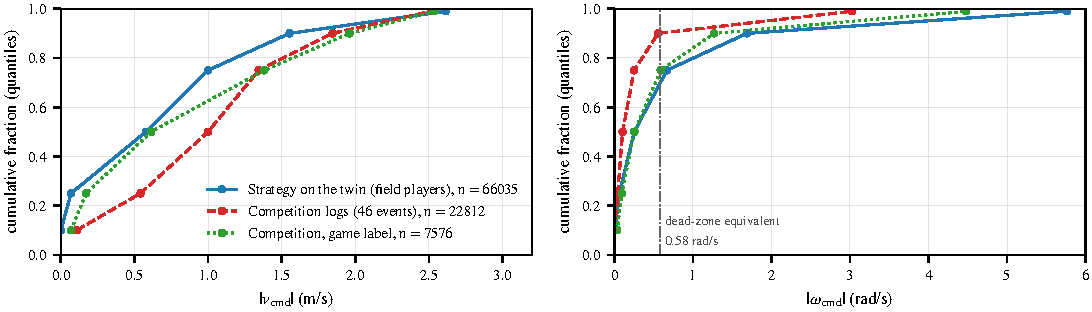
\includegraphics[width=\textwidth]{fig_journal_closed_loop.pdf}
  \caption{Commands of the team's strategy playing against the twin, against the competition logs: cumulative distributions of the commanded speed and yaw rate. Vertical line: body yaw rate equivalent to the firmware per-wheel dead zone.}
  \label{fig:closed}
\end{figure*}

% ==============================================================================
% tab_journal_closed_loop: generated by `dtssl analysis run journal_tables` (dtssl.analysis.journal_tables).
% Do not edit by hand: re-run the generator. Sources:
%   results/closed_loop_stats_20260907_2137.json
%   results/CHANGELOG.md 2026-09-07 21:37 (post hoc game-label reading)
% ==============================================================================
% Needs \usepackage{booktabs,adjustbox}.
\begin{table*}[t]
\centering
\caption{Closed-loop plausibility: what the strategy commands when it plays against the twin.}
\label{tab:closed-loop}
\small
\begin{adjustbox}{max width=\textwidth}
\begin{tabular}{lccc}
\toprule
& strategy on the twin (field players) & competition pool (46 events) & competition, game label \\
\midrule
samples at 60 Hz & 66035 & 22812 & 7576 \\
$|v_{\mathrm{cmd}}|$ median (m/s) & 0.578 & 1.000 & 0.614 \\
$|v_{\mathrm{cmd}}|$ 90th percentile (m/s) & 1.554 & 1.846 & 1.962 \\
$|\omega_{\mathrm{cmd}}|$ median (rad/s) & 0.251 & 0.104 & 0.254 \\
$|\omega_{\mathrm{cmd}}|$ 90th percentile (rad/s) & 1.687 & 0.556 & 1.269 \\
$|\omega_{\mathrm{cmd}}| < 0.58$ rad/s (\%) & 71.8 & 90.5 & 74.5 \\
dead zone alters / zeroes the command (\%) & 27.3 / 7.8 & 16.0 / 2.6 & 31.7 / 6.7 \\
idle (\%) & 12.6 & 1.4 & 3.6 \\
$|v_{\mathrm{cmd}}| > 2.9$ m/s (\%) & 0.31 & 0.01 & 0.01 \\
\midrule
$W_1$ distance of $|v|$ / $|\omega|$ to the session & -- & 0.326 / 0.387 & 0.179 / 0.127 \\
pre-registered plausibility criteria met & -- & 2/5 & 5/5 (post hoc) \\
\bottomrule
\end{tabular}
\end{adjustbox}

\vspace{2pt}
\parbox{\linewidth}{\footnotesize Commands of the team's real strategy closing the loop on the twin (recorded session, goalkeeper excluded) against the competition logs on the same 60 Hz grid. The pre-registered reference was the whole pool; 28 of its 46 events are scripted maneuvers, so the comparison with the game label is reported as post hoc.}
\end{table*}


\pending{text of the section.}
